\documentclass[conference]{IEEEtran}

\usepackage[utf8]{inputenc}
\usepackage[T1]{fontenc}
\usepackage{cite}
\usepackage{graphicx}
\usepackage{array}
\usepackage{tabularx}
\usepackage{booktabs}
\usepackage{url}
\usepackage[hidelinks]{hyperref}
\usepackage{tikz}
\usetikzlibrary{arrows.meta, positioning, fit, shapes.misc}
\usepackage{listings}
\usepackage{xcolor}
\usepackage{microtype}
\usepackage{enumitem}
\urlstyle{same}
\raggedbottom
\setlength{\emergencystretch}{2em}
\hbadness=10000
\hfuzz=10pt

\lstdefinestyle{code}{
  basicstyle=\scriptsize\ttfamily,
  breaklines=true,
  frame=single,
  columns=fullflexible,
  keepspaces=true,
  showstringspaces=false,
  xleftmargin=1mm,
  xrightmargin=1mm
}

\begin{document}
\hfuzz=10pt
\hbadness=10000
\setlist[itemize]{leftmargin=*, itemsep=1pt, topsep=2pt}
\setlist[enumerate]{leftmargin=*, itemsep=1pt, topsep=2pt}

\title{Cloud Rehosting for Cross-Platform Access to a Native Windows Desktop Application: A Case Study of GAMA Animation Engine}

\author{
\IEEEauthorblockN{Axelle Chandra, Muhammad Dafa 'Izzul Iman A., Muhammad Dhiwaul Akbar,\\
Dhimas Early Oceandy, Hammam Muhammad Yazid}
\IEEEauthorblockA{Department of Computer Science and Electronics\\
Faculty of Mathematics and Natural Sciences, Universitas Gadjah Mada\\
Yogyakarta, Indonesia}
}

\maketitle

\begin{abstract}
GAMA Animation Engine (GAE), a core component of Gamatutor, is a native Windows desktop application used to create and play simple tutorial animations. Its desktop-based architecture creates accessibility limitations because users normally need a compatible Windows environment and local installation before they can use the application. This project addresses that problem by rehosting GAE in a cloud-based environment and exposing it through browser-based remote access. The implemented architecture uses Amazon Elastic Compute Cloud (EC2) with two virtual machines: a Linux EC2 instance running Apache Guacamole as an HTML5 remote desktop gateway and a Windows EC2 instance running the GAE application. Users access the system through a web browser, while Apache Guacamole translates the browser session into an RDP connection to the Windows server. The result shows that GAE can be used from different operating systems without local installation and without significant modification to the original application source code. Although the solution is not a full cloud-native redesign, it successfully improves accessibility, simplifies user access, and demonstrates that rehosting is a practical migration approach for native Windows desktop applications that need cross-platform browser-based availability.
\end{abstract}

\begin{IEEEkeywords}
cloud computing, rehosting, legacy application, Apache Guacamole, AWS EC2, Remote Desktop Protocol, cross-platform access, GAMA Animation Engine
\end{IEEEkeywords}

\section{Introduction}

Cloud computing enables software to be accessed without depending entirely on local hardware and local installation. However, many useful applications are still designed as native desktop applications, especially older academic or institutional software that was originally built for a specific operating system. GAMA Animation Engine (GAE), part of the Gamatutor project, is one example. The original application is a Windows desktop application that includes tools such as TutorialGenerator and PlayerAnimasi for creating and playing tutorial animation content.

The main problem addressed in this project is not the absence of application functionality, but limited accessibility. In its original form, GAE is easier to use when the user has a compatible Windows device and performs local application setup. This creates barriers for users who use macOS, Linux, Chromebook, or other devices that do not directly run Windows desktop applications. It also makes the application less convenient because every user device needs its own installation and environment configuration.

This project therefore focuses on improving accessibility for a native Windows desktop application. Instead of rewriting GAE into a web application, the project keeps the original application behavior and moves the execution environment to the cloud. Users only need a browser, while the application runs on a Windows server in the cloud. This approach supports cross-platform usage and reduces local installation requirements.

The objective of this project is to design, implement, and evaluate a cloud rehosting architecture that allows GAE to be accessed through a browser. The final system uses Apache Guacamole as a web-based remote access gateway and AWS EC2 as the cloud infrastructure. The project also documents the deployment process, the weekly progress, and the use of AI assistance in preparing the final deliverables.

\section{Methods}

\subsection{Application and Problem Analysis}

GAE is treated as a native Windows desktop application. Based on the initial project analysis, the application is built using Delphi/Object Pascal with the Visual Component Library (VCL), runs as a standalone Windows application, and depends on local files such as animation files, images, and audio assets. These characteristics make the application strongly tied to the Windows desktop environment.

The accessibility problem can be summarized as follows. First, users need a compatible Windows environment to run the application directly. Second, the application must be installed or prepared on each local device. Third, users on non-Windows operating systems face additional barriers. Fourth, the local deployment model does not provide a simple centralized access point. Therefore, the project requires a deployment model that preserves the original Windows application while making it available through a universal interface: the web browser.

\subsection{Migration Strategy}

The selected migration strategy is rehosting, also known as lift-and-shift. Rehosting was selected because the project goal is to improve accessibility without changing the main behavior of the original application. In this approach, the application remains a Windows desktop application, but the runtime environment is moved from a local machine to a cloud-based Windows server.

This strategy is suitable for the project for three reasons. First, it avoids rewriting the application into a web application, which would require significant redevelopment. Second, it supports the original application environment by using Windows EC2 as the host. Third, it enables browser-based access by placing Apache Guacamole in front of the Windows environment. As a result, users do not interact directly with the Windows server through a traditional RDP client; instead, they access the remote desktop session from a standard web browser.

\subsection{Target Architecture}

The target architecture consists of three main layers: the client layer, the gateway layer, and the target application layer. The client layer is the user's device and web browser. The gateway layer is a Linux EC2 instance running Apache Guacamole, guacd, and a database service. The target application layer is a Windows EC2 instance where GAE is installed and executed.

\begin{figure*}[t]
\centering
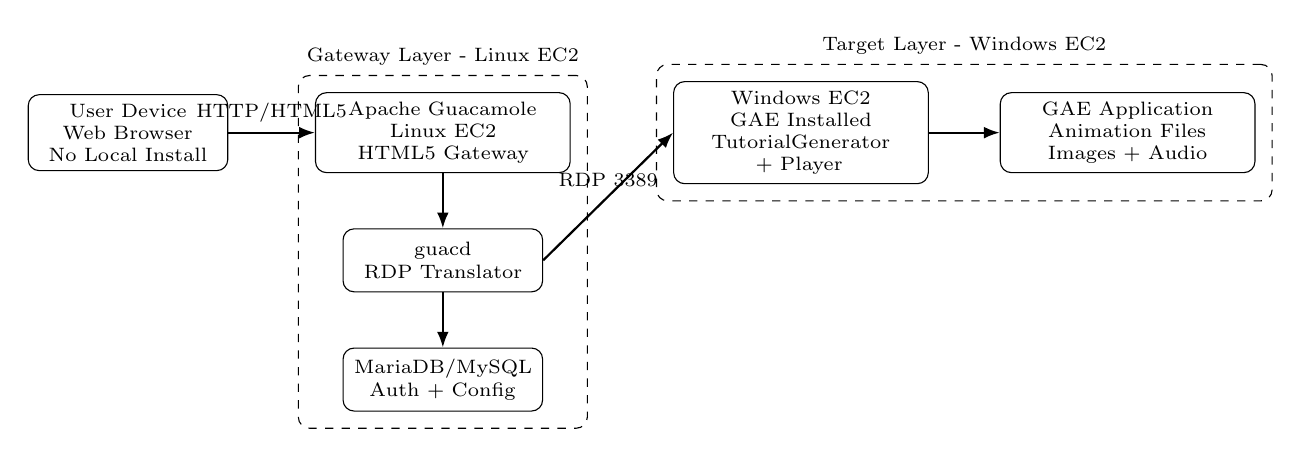
\begin{tikzpicture}[
  font=\scriptsize,
  box/.style={draw, rounded corners, align=center, minimum height=0.8cm, text width=2.3cm},
  widebox/.style={draw, rounded corners, align=center, minimum height=0.8cm, text width=3.0cm},
  layer/.style={draw, dashed, rounded corners, inner sep=6pt},
  arrow/.style={-{Latex[length=2mm]}, thick}
]

\node[box] (user) {User Device\\Web Browser\\No Local Install};

\node[widebox, right=1.1cm of user] (guac) {Apache Guacamole\\Linux EC2\\HTML5 Gateway};
\node[box, below=0.7cm of guac] (guacd) {guacd\\RDP Translator};
\node[box, below=0.7cm of guacd] (db) {MariaDB/MySQL\\Auth + Config};

\node[widebox, right=1.3cm of guac] (win) {Windows EC2\\GAE Installed\\TutorialGenerator + Player};
\node[widebox, right=0.9cm of win] (app) {GAE Application\\Animation Files\\Images + Audio};

\draw[arrow] (user) -- node[above]{HTTP/HTML5} (guac);
\draw[arrow] (guac) -- (guacd);
\draw[arrow] (guacd) -- (db);
\draw[arrow] (guacd.east) -- node[above]{RDP 3389} (win.west);
\draw[arrow] (win) -- (app);

\node[layer, fit=(guac)(guacd)(db), label=above:{Gateway Layer - Linux EC2}] {};
\node[layer, fit=(win)(app), label=above:{Target Layer - Windows EC2}] {};

\end{tikzpicture}
\caption{Target cloud rehosting architecture for browser-based access to GAE.}
\label{fig:architecture}
\end{figure*}

Figure~\ref{fig:architecture} shows the target architecture. The browser does not run GAE directly. Instead, the browser renders an HTML5 remote desktop session provided by Apache Guacamole. Guacamole communicates with guacd, and guacd establishes an RDP session to the Windows EC2 instance. The Windows EC2 instance hosts the original GAE desktop environment.

\subsection{Infrastructure Components}

Table~\ref{tab:components} summarizes the main infrastructure components used in the prototype. The architecture separates user access from the Windows application host. This separation allows the Windows instance to be protected from direct public exposure while the Guacamole gateway becomes the browser-facing access point.

\begin{table}[!t]
\centering
\caption{Infrastructure Components}
\label{tab:components}
\begin{tabularx}{\columnwidth}{p{2.2cm}X}
\toprule
\textbf{Component} & \textbf{Role} \\
\midrule
User browser & Accesses GAE without local installation. \\
Linux EC2 & Hosts the Apache Guacamole gateway. \\
Apache Guacamole & Provides browser-based remote desktop access. \\
\texttt{guacd} & Translates the Guacamole protocol to RDP. \\
MariaDB/MySQL & Stores Guacamole users, connections, and configuration. \\
Windows EC2 & Runs the original GAE desktop application. \\
RDP & Connects Guacamole to the Windows desktop environment. \\
\bottomrule
\end{tabularx}
\end{table}

\subsection{Deployment Procedure}

The deployment process was divided into local proof-of-concept testing and cloud implementation. The local proof of concept was used to verify that the application could run inside a virtualized Windows environment and could be accessed through RDP. After that, the cloud infrastructure was prepared on AWS.

The cloud deployment process consists of the following steps:

\begin{enumerate}
    \item Prepare an AWS account and configure a project budget to control cost.
    \item Create a Virtual Private Cloud (VPC), subnet, route table, and internet gateway.
    \item Launch a Linux EC2 instance to host Apache Guacamole.
    \item Launch a Windows EC2 instance to run the GAE application.
    \item Configure security groups so that browser users access Guacamole through port 8080, while RDP access to Windows is limited to the internal VPC or the Guacamole gateway.
    \item Install Docker and Docker Compose on the Linux EC2 instance.
    \item Deploy Guacamole, \texttt{guacd}, and database services using the deployment repository.
    \item Install GAE on the Windows EC2 instance using the original Gamatutor application repository.
    \item Configure a Guacamole RDP connection to the Windows EC2 instance.
    \item Test browser-based access from the user device to the cloud-hosted GAE application.
\end{enumerate}

\subsection{Repositories}

Two GitHub repositories were used in the project. The first repository is the original GAE/Gamatutor application repository. It contains the application artifact and source materials for GAE. The second repository is the deployment configuration repository prepared for this cloud computing project. It contains Docker-based configuration files used to deploy Apache Guacamole and its supporting services.

Separating these repositories is important because the project does not claim to create GAE from scratch. The main contribution of this project is the rehosting environment and access architecture. The original application remains the application being hosted, while the deployment repository supports the cloud access layer.

\section{Results}

\subsection{Local Proof of Concept}

Before deploying the system to AWS, the team tested a local virtual machine environment. The purpose was to verify that GAE could run in a virtualized Windows environment and that the desktop environment could be accessed remotely. In the weekly progress presentation, the team reported that the application had been installed inside a local virtual machine and could be accessed through RDP. At this stage, Guacamole installation and integration still needed further work.

The local proof of concept confirmed that remote access was feasible for the application. This result became the basis for moving to the cloud deployment stage, where the same idea was implemented using EC2 instances.

\subsection{Cloud Rehosting Result}

The final cloud implementation successfully rehosted GAE using the architecture shown in Fig.~\ref{fig:architecture}. The user accesses the system from a browser, the request is handled by Apache Guacamole running on Linux EC2, and the GAE desktop environment is delivered from a Windows EC2 instance through RDP. The team reported the final progress as 100\% after the cloud access architecture was completed.

The final implementation achieved the main accessibility goals. First, users no longer need to install GAE on their local devices. Second, users from different operating systems can access the application as long as they have a compatible browser. Third, the Windows-specific runtime requirement is moved to the cloud. Fourth, the user-facing access method becomes simpler because the browser becomes the main interface.

\subsection{Functional Testing}

Functional testing was performed by comparing expected behavior in the local and cloud environments. The tests focused on whether the application could be opened, whether the remote desktop connection worked, and whether the browser-based access flow could reach the Windows EC2 desktop.

\begin{table}[!t]
\centering
\caption{Functional Testing Summary}
\label{tab:testing}
\begin{tabularx}{\columnwidth}{p{0.45cm}X p{1.2cm}}
\toprule
\textbf{No.} & \textbf{Test Case} & \textbf{Status} \\
\midrule
1 & Run GAE in local Windows environment. & Passed \\
2 & Access virtualized Windows environment through RDP. & Passed \\
3 & Deploy Guacamole gateway on Linux EC2. & Passed \\
4 & Connect Guacamole to Windows EC2 through RDP. & Passed \\
5 & Access Windows EC2 from a browser through Guacamole. & Passed \\
6 & Run GAE on the Windows EC2 instance. & Passed \\
7 & Use browser-only access without installing GAE locally. & Passed \\
\bottomrule
\end{tabularx}
\end{table}

Table~\ref{tab:testing} shows that the system passed the main functional tests required for the project. The most important result is not that GAE was changed internally, but that the original Windows application could be accessed through a browser-based cloud environment.

\subsection{Deployment Configuration Result}

The deployment repository was used to organize the Guacamole gateway setup. The Docker-based configuration includes Guacamole, \texttt{guacd}, and a database. The Guacamole service exposes port 8080 during the prototype stage, while \texttt{guacd} handles remote desktop protocol translation. The database stores authentication data and connection configuration.

The use of Docker Compose simplified the gateway setup because the required services could be started consistently on the Linux EC2 instance. However, the prototype configuration also revealed security concerns, such as the use of simple credentials and hardcoded secrets in configuration files. These issues are discussed as limitations in Section~IV.

\subsection{Video Demonstration Attachments}

The final deliverables require two video demonstrations. The first video demonstrates GAE running in the local or on-premise environment. The second video demonstrates GAE running through the cloud server using browser-based access via Guacamole. These videos should be submitted as separate attachments or linked in the appendix.

\section{Discussion}

\subsection{Accessibility Improvement}

The main value of the project is improved accessibility. In the original model, users need a Windows-compatible local environment. In the rehosted model, users only need a browser. The actual Windows execution environment is moved to the cloud, while Guacamole presents the remote session through an HTML5 interface. This makes the application easier to access from macOS, Linux, Windows, and potentially other browser-capable devices.

This approach is especially useful for desktop applications that are still valuable but difficult to distribute widely. Instead of asking every user to install and configure the application, the administrator prepares one centralized environment. Users then access that environment remotely.

\subsection{Why Rehosting Was Appropriate}

Rehosting was appropriate because the goal was not to redesign the application, but to make it more accessible. Rewriting GAE as a web application would require significant changes to the source code, user interface, storage behavior, and runtime model. Containerizing the Windows desktop GUI directly would also not solve the user interaction problem as simply as browser-based remote desktop access.

By using Windows EC2, the project preserves the original execution environment. By using Apache Guacamole, the project provides a browser interface. The combination of these two components directly matches the project objective: cross-platform, no-install access to a native Windows desktop application.

\subsection{Limitations}

Although the system improves accessibility, it has several limitations. First, the system is still dependent on a Windows EC2 instance. This means that the application is not fully cloud-native and still requires a desktop runtime. Second, the user experience depends on network quality and remote desktop latency. Third, the prototype still requires careful cost management because cloud instances may generate cost when running continuously. Fourth, multi-user access may require additional configuration, depending on how many simultaneous users need to access the application.

The deployment configuration also needs improvement before production use. Prototype credentials and hardcoded secrets should be replaced with environment variables or a proper secret management mechanism. The Guacamole interface should also be placed behind HTTPS, and security groups should restrict administrative access.

\subsection{Security Considerations}

The architecture provides a better security model than exposing the Windows RDP server directly to the public internet. Ideally, the Windows EC2 instance should only accept RDP traffic from the Guacamole gateway inside the VPC. The public-facing component should be the Guacamole web interface, protected by authentication and secure transport.

For a production deployment, several improvements are recommended. First, enable HTTPS for the Guacamole interface using a domain and TLS certificate. Second, use stronger credentials and avoid committing secrets to the repository. Third, restrict SSH access to trusted administrator IP addresses. Fourth, monitor instance usage and logs. Fifth, consider backup and snapshot policies for the Windows EC2 instance.

\subsection{Cost and Operational Considerations}

The project used AWS budget configuration to control spending during the experiment. This is important because rehosting desktop applications on cloud virtual machines can be more expensive than lightweight web hosting. The Windows EC2 instance is the main cost component because it must provide a graphical desktop environment.

For long-term usage, the system should evaluate instance scheduling, automatic shutdown, reserved capacity, or alternative remote application delivery models. These improvements can reduce operational cost while maintaining accessibility.

\section{Conclusion}

This project successfully rehosted GAE, a native Windows desktop application, into a cloud-based environment to improve accessibility. The final architecture uses Apache Guacamole on Linux EC2 as a browser-based remote desktop gateway and Windows EC2 as the application host. Through this design, users can access GAE from different operating systems without installing the application locally.

The result shows that rehosting is a practical strategy for improving access to native desktop applications that are difficult to distribute across platforms. The project does not transform GAE into a cloud-native application, but it achieves the main goal of browser-based, cross-platform, no-install access. Future improvements should focus on stronger security, HTTPS deployment, better secret management, cost optimization, and multi-user access management.

\begin{thebibliography}{00}

\bibitem{ieee-template}
IEEE, ``IEEE Conference Templates,'' IEEE Author Center. [Online]. Available: \url{https://www.ieee.org/conferences/publishing/templates}

\bibitem{imrad}
T. Dube, ``IMRAD In Science: The Importance a Format Can Have,'' Medium, 2015. [Online]. Available: \url{https://medium.com/literacy-discourse/imrad-in-science-4a29e6c63ccc}

\bibitem{guacamole}
Apache Software Foundation, ``Apache Guacamole Manual,'' Apache Guacamole Documentation. [Online]. Available: \url{https://guacamole.apache.org/doc/gug/}

\bibitem{aws-ec2}
Amazon Web Services, ``Amazon EC2 Documentation,'' AWS Documentation. [Online]. Available: \url{https://docs.aws.amazon.com/ec2/}

\bibitem{rdp}
Microsoft, ``Remote Desktop Protocol,'' Microsoft Learn. [Online]. Available: \url{https://learn.microsoft.com/}

\bibitem{gamatutor}
Gamatutor, ``gamatutor/gamatutor: GAE -- Engine Pembuat dan Player Animasi Tutorial Sederhana,'' GitHub. [Online]. Available: \url{https://github.com/gamatutor/gamatutor}

\bibitem{deployment-repo}
EarlyOcean, ``cloud-computing-final-project,'' GitHub. [Online]. Available: \url{https://github.com/EarlyOcean/cloud-computing-final-project}

\end{thebibliography}

\appendices

\section{Weekly Progress}

Table~\ref{tab:weekly} summarizes the weekly progress submitted during the project.

\begin{table*}[!t]
\centering
\caption{Weekly Progress Summary}
\label{tab:weekly}
\begin{tabularx}{\textwidth}{p{0.8cm}p{3.1cm}X p{2.0cm}}
\toprule
\textbf{Week} & \textbf{Activity} & \textbf{Output} & \textbf{Status} \\
\midrule
1 & Project topic selection and application analysis & Selected GAE/Gamatutor as the legacy Windows desktop application for rehosting. & Completed \\
2 & Requirement and problem analysis & Identified the main problem as limited accessibility due to Windows dependency and local installation. & Completed \\
3 & Local proof of concept & Created a local VM using VirtualBox, installed the application, and verified RDP access. & 40\% progress \\
4 & Cloud architecture design & Designed the architecture using Linux EC2 for Guacamole and Windows EC2 for GAE. & Completed \\
5 & AWS setup and EC2 provisioning & Prepared AWS budget, VPC, Linux EC2, and Windows EC2 instances for cloud implementation. & Completed \\
6 & Guacamole deployment and integration & Deployed Apache Guacamole, guacd, and database services on Linux EC2 and connected them to Windows EC2. & Completed \\
7 & Final testing, documentation, and demonstration & Verified browser-based access to GAE through Guacamole and prepared final report, appendix, and video demonstrations. & 100\% progress \\
\bottomrule
\end{tabularx}
\end{table*}

\section{Step-by-Step Deployment Documentation}

This appendix provides a concise version of the technical deployment steps used in the rehosting process.

\subsection{Prepare AWS Account and Budget}

Create or access an AWS account. Configure AWS Budget to monitor spending during the project. This step is important because running EC2 instances continuously can generate cost.

\subsection{Create VPC and Network Components}

Create a VPC, subnet, route table, and internet gateway. The VPC is used to place both the Linux EC2 and Windows EC2 instances in the same cloud network. The Windows instance should be reachable from the Guacamole gateway, but it should not be exposed directly to the public internet through open RDP access.

\subsection{Launch Linux EC2 for Guacamole}

Launch an Ubuntu Linux EC2 instance. Attach a security group that allows SSH from the administrator's IP address and HTTP access to the Guacamole prototype port. In a production configuration, port 8080 should be placed behind HTTPS using a reverse proxy.

\begin{lstlisting}[style=code,caption={Example Linux EC2 access command}]
ssh -i /path/to/keypair.pem ubuntu@<linux-ec2-public-ip>
\end{lstlisting}

\subsection{Install Docker and Docker Compose}

Install Docker and Docker Compose on the Linux EC2 instance. The exact commands may vary depending on the operating system image.

\begin{lstlisting}[style=code,caption={Example Docker installation commands}]
sudo apt update
sudo apt install -y docker.io docker-compose-v2
sudo systemctl enable docker
sudo systemctl start docker
sudo usermod -aG docker ubuntu
\end{lstlisting}

\subsection{Deploy Guacamole Services}

Clone the deployment repository and start the Docker Compose services. The project repository contains the configuration for Guacamole, guacd, database, and supporting services.

\begin{lstlisting}[style=code,caption={Deploying Guacamole services}]
git clone https://github.com/EarlyOcean/cloud-computing-final-project.git
cd cloud-computing-final-project
mkdir -p init data drive record
docker compose up -d
\end{lstlisting}

After the containers are running, verify the deployment.

\begin{lstlisting}[style=code,caption={Checking running containers}]
docker compose ps
\end{lstlisting}

Open the Guacamole web interface from a browser using the Linux EC2 public IP address and port 8080.

\begin{lstlisting}[style=code,caption={Prototype Guacamole URL format}]
http://<linux-ec2-public-ip>:8080/guacamole/
\end{lstlisting}

\subsection{Launch Windows EC2 for GAE}

Launch a Windows Server EC2 instance. Configure the security group so that RDP port 3389 is reachable only from the Guacamole gateway or from the internal VPC, not from the entire public internet. Retrieve the Windows administrator password using the selected key pair.

\subsection{Install GAE on Windows EC2}

Download the original Gamatutor/GAE application artifact from the official repository. Install or copy the required application files to the Windows EC2 instance. Verify that the application components such as TutorialGenerator and PlayerAnimasi can be executed in the Windows environment.

\begin{lstlisting}[style=code,caption={Original application repository}]
https://github.com/gamatutor/gamatutor
\end{lstlisting}

\subsection{Create Guacamole RDP Connection}

Log in to Guacamole as an administrator and create a new RDP connection. Configure the connection using the private IP address of the Windows EC2 instance, port 3389, and the Windows login credentials. After saving the connection, open it from the Guacamole dashboard to verify that the Windows desktop appears in the browser.

\subsection{Run GAE Through Browser}

From the browser-based Guacamole session, run the GAE application on the Windows EC2 desktop. The user should be able to interact with GAE without installing it locally. This verifies the main goal of the project: cross-platform browser-based access to a native Windows desktop application.

\section{Source Code and Deployment Repositories}

The project uses two repositories:

\begin{itemize}
    \item Original GAE/Gamatutor application repository: \url{https://github.com/gamatutor/gamatutor}
    \item Deployment configuration repository: \url{https://github.com/EarlyOcean/cloud-computing-final-project}
\end{itemize}

The original repository contains the GAE/Gamatutor application artifact and source materials. The deployment repository contains Docker-based configuration used to deploy the Guacamole access gateway. In this project, the original GAE application was not significantly modified. The main work was the preparation of the cloud rehosting environment.

\section{Video Demonstration Links}

The final deliverables include two demonstration videos:

\begin{itemize}
    \item Video 1: Local/on-premise GAE demonstration. Link: \textit{to be inserted}.
    \item Video 2: Cloud-hosted GAE demonstration through Apache Guacamole. Link: \textit{to be inserted}.
\end{itemize}

\section{AI Declaration}

AI-based tools were used to support the preparation of the final deliverables. ChatGPT was used to help organize the report structure, refine academic wording, prepare the IEEE-style LaTeX draft, and improve the clarity of the appendix documentation. The authors reviewed and edited the generated content to match the actual project implementation.

The AI assistance was used for writing support and documentation organization. It was not used to fabricate project results. The system architecture, implementation process, repository links, progress reports, and demonstration requirements were based on the actual project work.

The following consolidated prompts represent the AI assistance used during report preparation:

\begin{enumerate}
    \item ``Create an IEEE-style final report outline using the IMRAD structure for a cloud computing project about rehosting GAMA Animation Engine, a native Windows desktop application, to improve cross-platform accessibility through browser-based access.''
    \item ``Draft the abstract, introduction, methods, results, discussion, and conclusion for a final report about rehosting GAE using Apache Guacamole, Linux EC2, Windows EC2, and RDP.''
    \item ``Revise the report narrative so the main focus is solving accessibility limitations of a Windows desktop application, enabling users from different operating systems to access it without local installation through a web browser.''
    \item ``Prepare a concise appendix containing weekly progress, deployment steps, repository links, video demonstration placeholders, and an AI declaration for the final deliverables.''
    \item ``Improve the LaTeX formatting so that the IEEE report is cleaner, easier to read, and suitable for Overleaf compilation.''
\end{enumerate}

\end{document}
